With these changes to Derby we have gained scalability, fault and partition tolerance and kept durability. This of course came with the cost of loosing atomicity\footnote{Cassandra provides atomicity at the row level, which is fine when doing separate inserts at a time, but is not good enough when performing batch inserts or transaction that affects multiple rows}, isolation and consistency (we have eventual consistency). 

In practical terms this means that transactions are not possible with this system. To overcome these limitations we built a distributed transaction system that takes advantage of Cassandra's peer to peer architecture and integrates with Derby.

\section{Algorithm}
The adopted algorithm (Alg. \ref{alg:good-run}) combines a mechanism of locks and a write ahead log with Cassandra's provided atomicity and idempotent operations.

\begin{algorithm}  
  \DontPrintSemicolon
  \SetKwInput{KwIn}{Require}
  \SetKwInput{KwOut}{Ensure}
  \KwIn{Lock(A,B)} \tcp*[l]{A and B are columns with random values}
  \Indp
    $A_{i} \gets Read(A)$ \;
    $B_{i} \gets Read(B)$ \;
    $TID \gets getUniqueID()$ \; 
    $Write(TID,R_{A})$ \tcp*{$R_{A}$ represents the row that holds A}
    $Write(TID,R_{B})$ \;
    $(A_{f},B_{f}) \gets compute(Ai,Bi)$ \;
    $Write((A_{f},B_{f}),T)$ \tcp*{T represents the row with id TID}
    $Write(A_{f},A)$ \;
    $Write(B_{f},B)B$ \;
  \Indm
  \KwOut{Unlock(A,B)}
 \caption{Transactional Model for Cassandra - Run without failures}
 \label{alg:good-run}
\end{algorithm}

Take in account that $A_{i}$, $A_{f}$, $B_{i}$ and $B_{f}$ are random values, that the \emph{compute} function represents all the operations in the transaction and that the operation in line 7 is atomic due to the guarantees given by Cassandra. Note that the \emph{Write} function takes two arguments, the tuple to be written and the place to write it (row, column, etc...). 

The write in line 7 defines the no return point, i.e. after this moment the changes are committed and will persist through failure, prior to this moment if the node fails for any reason, all the updates will be lost and the transaction will have to be replayed.

\subsection{API}
The basic Cassandra operations (\emph{get}, \emph{put} and \emph{delete}) were redefined and all interactions with the cluster during transactions must pass through the transactional system. This is of major importance since Cassandra does not possess a versioning system and as such, all operations that would alter the data must wait until the commit for the updates to be pushed to disk, or else the \textbf{consistency} property will be broken. For instance, if a transaction writes to a column X before entering the commit stage, the next transaction to read from X will read an inconsistent value and will have no way of reverting it to the previous consistent state.

To summarize, the behavior of these operations is defined as follows:

\begin{description}
	\item[\emph{get(keyspace, columnFamily, rowKey, columnName, consistencyLevel)}] Will first apply the recover mechanism (Section \ref{sec:rec_fail}) to the row and then get the desired data from the data store
	\item[\emph{put(keyspace, columnFamily, rowKey, columnName, value)}] Will write the new value to memory in the form of a Cassandra \emph{Column}, and wait until commit to see the changes pushed to disk
	\item[\emph{delete(keyspace, columnFamily, rowKey, columnName, timestamp)}] Works as the \emph{put} operation, but always writes the same special value (\emph{$\textunderscore\textunderscore$delete$\textunderscore\textunderscore$}) 
\end{description}  

We also provide some extra methods that derive from this, such as the \emph{get\_range} and \emph{get\_slice} methods that allow to get more that one value with only one request to the datastore, in order to optimize range queries. For simplicity, a \emph{put} can receive a \emph{Column} object, instead of a column name and value which also allows for the timestamp to be created by the application.

\subsubsection{Deletes}
Deleting is a special operation because if a delete occurs previous updates must not be preserved. There are three kinds of deletions contemplated by our system, of a column, a row or a keyspace and each of them must be treated in a different way.

\begin{description}
	\item[Delete column] This is the simpler and behaves as explained before, by doing an update with a special value
	\item[Delete row] The mechanism is similar to that of deleting a column, but the special value (\emph{$\textunderscore\textunderscore$delete$\textunderscore\textunderscore$}) is written to the column's name and not its value so when committing everything with a timestamp previous to the one of the column will be deleted
	\item[Delete keyspace] There is no actual method for deleting a keyspace through our system, you must use Cassandra's API for that, what the system does is check if the keyspace exists before performing the updates on a commit, and if it does it is aborted. If for some reason the transaction does not commit nor abort (fails), there might be columns left with no pointer to them (ghost columns) that can be cleaned with a Garbage Collector set to act at a specific time. This is a similar mechanism to the one implemented by Cassandra.  
\end{description}

\section{Caching}
The only way to perform a transaction in a system like Cassandra that does not provide \ac{mvcc} is to lock (Section \ref{sec:locks}) the data you need in order to prevent it from changing, since data cannot have multiple versions and when it is written there is no way of rolling back. Alongside with this, all the data changes made by the transaction itself must be cached and taken in account at every statement.

\subsection{Read-your-own-writes consistency}
One possible eventual consistency property is read-your-own-writes consistency, meaning a process is guaranteed to see the writes it has made when it does reads. Since puts and deletes are not committed until the end of the transaction, when performing a get (read) it must take in account those values that are in memory but not yet committed and merge them with the values it gets from the \ac{vlsd}. This will provide the read-your-own-writes property which is crucial to maintain the consistency of the system.

\subsection{Merging data from disk and memory}
As stated earlier our \ac{api} provides three different types of \emph{get} methods. One for reading a single column, one for reading an entire row or a slice (certain columns) of a row and one to read a range of rows that can possibly be sliced. Each of these methods uses the cache in a different ways, in order to retrieve the intended data.

The first one is trivial, since only one column is asked for, if it is in memory then it is the newer value and it is returned. If it is not in memory, then it must be fetched from disk and then returned.

The second one consists in fetching the row from disk and merge those values with the ones cached, with the following restrictions:
\begin{itemize}
	\item If there has been a deletion that affects the column\footnote{This deletion can be of an entire column family, a row or simply that column} which has occurred after the insertion of said column (temporal order is achieved through the columns' timestamps), then the column is not valid and must not be retrieved
	\item A cached column's value always prevails to the ones coming from disk. This is true since we have made sure, through locking, that the values on disk do not change during the transaction
\end{itemize}

The last method for reading data interacts with the cache by first getting the range of rows from disk, performing the same range query to the cached data and merge them according to the same principles explained above.

There is one other step that is common to all the methods and must be performed before fetching actual data from disk, which is the recovery from failure of a row that is described by the algorithm \ref{alg:recovery-run}.

\section{Locks}
\label{sec:locks}
Before the transaction can start, it must acquire the locks for the rows or entire tables (in read only mode or not) it is going to use. We use a readers-writer lock mechanism, that provides two kinds of locks, read and write. This mechanism allows concurrent access to multiple threads for reading but restricts access to a single thread for writes to the resource.

The actual lock mechanism works firstly by asking for a lock on the table for \emph{any\_or\_all}, when attempting to lock the entire table for writing this is a write lock, otherwise it is a read lock. In the second case there is a second step of asking for locks on the rows we need, since there can be many concurrent transactions with read locks on the same table at the same time. This means that all transactions can pass on to ask for locks on the rows, unless there is another waiting to lock the whole table.

A lock is represented by a Path class, that encapsulates the path to the lock as well as its type (table lock or not) and provides the necessary primitives to work with it. 

Still this mechanism is not enough because it does not prevent deadlocks\footnote{If two threads want locks A and B, and one of them gets A and the other B, they will both be waiting on the other, which is the definition of a deadlock}. In order to do this, there has to be a globally accorded way of ordering the paths of the locks, for this we first compare the nesting of the path (table locks are less nested and therefore are sorted first), then we compare the actual name of the table\footnote{using Java strings default compareTo method} and at last, in the case of rows of the same table, we compare the name of the row. This comparison in done with a Comparator class, which provides a way to change how paths are compared without changing the code of the actual system.

\subsection{Zookeeper}
\label{sec:zoo}
ZooKeeper is a centralized service for maintaining configuration information, naming, providing distributed synchronization, and providing group services~\cite{zooDef}. We use the naming services of Zookeeper to maintain our locks, since it allows distributed processes to coordinate with each other through a shared hierarchal namespace which is organized similarly to a standard (unix) file system (Fig. \ref{fig:zoo_namespace}). 

\begin{figure}[htb]
  \begin{center}
    \leavevmode
    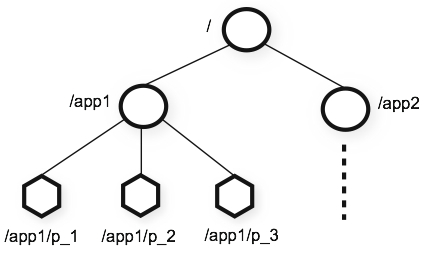
\includegraphics[width=0.7\textwidth]{images/zknamespace.jpg}
  \end{center}
  \caption{ZooKeeper's Hierarchical Namespace}
  \label{fig:zoo_namespace}
\end{figure}

Other than the ease of use, Zookeeper is intended to be replicated and provides total order of updates in the cluster~\cite{zooDoc} which are properties we need to implement the locks~\cite{zooLocks}. Also, it supports the concept of \emph{watches}, that are callbacks registered by the client for when certain events take place, for example when a node is deleted. This is a useful feature when implementing locks so that clients do not have to busy wait\footnote{When busy waiting a client thread will always be polling the server in order to know if the event has occured}.

\subsection{Cages}
\label{sec:cages}
According to the creator's blog~\cite{cages}, Cages is a Java library that provides distributed synchronization functionality by using the services of a ZooKeeper server or cluster. 

Cages offers three types of locking, ZkReadLock, ZkWriteLock and ZkMultiLock. As can be inferred by the names, these represent a read lock and write lock, and the multi lock is an attempt to provide a primitive for acquiring multiple locks at the same time. This primitive proved to be ineffective as it is not atomic, it is the equivalent to try to acquire multiple locks one at a time and therefore is useless for our implementation since it can lead to deadlocks.

The locks are represented by a string in the form used by ZooKeeper (Fig. \ref{fig:zoo_namespace}). An example of how to acquire a write lock is shown in code sample \ref{lst:cageslocks}.
 
\lstset{
  language=Java, 
  caption=Acquiring a lock with Cages, 
  label=lst:cageslocks,
}
\definecolor{shadecolor}{gray}{0.95}


\begin{shaded}
\begin{lstlisting}
void methodX() {
    ZkWriteLock lock = new ZkWriteLock("/path/to/lock");
    lock.acquire();
    try {
        // The code
    } finally {
        lock.release();
    }
}
\end{lstlisting}  
\end{shaded} 

Note that the path for the lock has no restrictions as long as it is followed through the whole application. Also, if a node fails and has a lock Cages will make sure it releases that lock after a certain amount of time of inactivity.

Since this locking systems stores nothing but meta data, i.e. the names of the locks that someone holds, and not the locks themselves, it is important that it is highly available and consistent or else the system itself may become inconsistent. For this, we use a zookeeper cluster with three nodes, which is enough for most workloads\cite{zooPerf}, and it is not desirable to scale ZooKeeper clusters beyond this number of nodes. The reason for this is that while adding nodes scales up read performance, write performance actually starts degrading because of the need to synchronize write operations across all members, and therefore clustering really offers availability rather than performance. 

If Zookeeper becomes a bottleneck there are two solutions, the one presented by Dominic Williams that is to run more than one ZooKeeper cluster and simply hash the locks' paths to particular clusters, and to use a feature introduced in Zookeeper 3.3, the \emph{Observers}.  

\subsubsection{ZooKeeper Observers}
Normal Zookeeper nodes connect to the cluster as voting members, meaning that they participate in the consensus, making it hard to scale out to a big number of clients. This happens because a write operation needs (in general) the agreement of at least half the voting nodes, increasing the cost of voting as nodes are added.

To address this problem, a new type of node is introduced, the observers. This nodes are members of the cluster that are not allowed to vote nor are aware of the voting algorithm, they only receive the results of the voting, other than this they function like normal nodes. 

Clients can connect and send read and write requests to them, which they redirect to the Leader and wait for the result of the vote. This allows many Observers to be added without harming the performance of the voting algorithm.

Other advantage of Observers is that as they are not critical to the function of the system, they can fail or be disconnected without harming the overall availability. This also means that these type of nodes can be on different data centers, providing faster (local) reads and diminishing the number of messages transmitted through the network in a write. \\ 

To sum up, the system uses a Zookeeper cluster alongside with the Cages library in order to provide table and/or row locking.

\section{Recovery from failure}
\label{sec:rec_fail}
The presented algorithm (Alg. \ref{alg:good-run}) only contemplates the case of a successful run, but it would be unrealistic to think that would always be the case. Therefore there is also a mechanism to recover from failures that is provided by a \ac{wal} technique.  

\subsection{Write-ahead Log}
The \ac{wal} technique used s represented by a super column family called \emph{Transactions\_WALog} that holds rows with the unique ids of the transactions as the row id.

In a system using \ac{wal}, all modifications are written to a log before they are applied which is a way of providing atomicity and durability.

Unlike relational databases where this is used in a checkpointing system, where if at some point there is a need for redoing operations all the logs in the \ac{wal} file are applied, in our system the logs are used on a need basis. What this means is that if there are some records in a transaction that could not be updated because of a failure, the update is redone at the time of the next read to that record's row.

One part of this technique is saving the data of the updates to the \ac{wal} column family (line 7, alg. \ref{alg:good-run}), the rest only takes places when something goes wrong and this data needs to be used. Lines 4 and 5 of the same algorithm are important because that \emph{TID} in each row is what allows the application to know when an error occurred and triggers the recovery algorithm (line 1, alg. \ref{alg:recovery-run}).
 

\begin{algorithm}
  \DontPrintSemicolon
  \KwIn{Path}
  \tcp*[l]{Path is a string in the form \emph{keyspace$\textunderscore\textunderscore$columnFamily$\textunderscore\textunderscore$rowKey}}
  \BlankLine
  \If{$lost$-$T \neq NULL$}
  {
	$TID \gets getVal(lost$-$T)$ \;
	$update\_columns \gets getOldRow(Path,TID,Transaction\_WALog)$ \;
	\ForEach{$column \in update\_columns$}
	{
	  $name \gets getName(column)$ \;
	  $path\_to\_column \gets Path + name$ \;
	  \tcp*[l]{Path gets to the row and name to the actual column}
	  $value \gets getVal(column)$ \;
	  $Write(value,path\_to\_column)$ \;
	}
	$Write(NULL,lost$-$T)$ \;
  }
 \caption{Transactional Model for Cassandra - Recover row after failure}
 \label{alg:recovery-run}
\end{algorithm}
 
This algorithm (Alg. \ref{alg:recovery-run}) is responsible for ensuring that if an update has been written to the log, then all subsequent reads to that record will reflect the update (\textbf{isolation}). The lost-T column exists in every row and has either nothing or the TID of the transaction it is in. This allows the system to know if there was an error in the middle of a transaction involving a given row, since the only way for an operation in a transaction other than its own to read that column is due to a previous error or the locking mechanism being broken (which should not happen). 

It then gets a TID from the lost-T column and uses it to get a set of columns to update, that are all the columns in the super column with the name given in $Path$ from the \emph{Transaction\_WALog} column family and the row with that TID as id. In the algorithm above, this is represented by the functions \emph{getVal} and \emph{getOldRow}, which get the value of a given column and the entire row information stored in the log for the row given by the $Path$, respectively.

Each of the columns retrieved from the log has the name of the column to be updated as name, and as value the corresponding value of the column. The value is gotten using the previously mentioned \emph{getVal} function and the name with the \emph{getName} function, the path is then constructed from the composition of the $Path$ variable that holds the names of the keyspace, column family and row to write to and the name of the column in that row, afterwards the value is written to that path.

To conclude it cleans the \emph{lost-T} column, which means the row is in a consistent state.

\section{Pre-processing difficult transactions}
The term difficult transaction was defined by Alexander Thomson and Daniel J. Abadi~\cite{Thomson:2010:CDD:1920841.1920855} when referring to transactions where it is impossible to request locks on every record it accesses immediately upon entering the system. Consider the example transaction proposed by them
\begin{align*}
U(x):& \\
&y \gets read(x)\\
&write(y)
\end{align*}
where x is a record’s primary key, y is a local variable, and write(y) updates the record whose primary key is y. It is obviously impossible for a transaction of type \emph{U} to request all the locks it is going to need, since some of them (in this case \emph{y}) depend on an operation that has not yet happened. 

They propose an approach to circumvent this problem, by partitioning difficult transactions into more than one, in this case it would be partitioned as such:
\begin{align*}
U_{1}(x):& \\
&y \gets read(x)\\
&newTransaction(U_{2}(x,y))
\end{align*}
and
\begin{align*}
U_{2}(x,y):&\\
&y' \gets read(x)\\
&if (y' \neq y)\\
&\qquad newTransaction(U_{2}(x,y'))\\
&\qquad abort()\\
&else\\
&\qquad write(y)
\end{align*}

So, it first gets the locks it does not yet know (a typical example of this would be the usage of indexes) and then starts the second transaction with all of the locks. This has to do a sanity check first, for the cases when the pre-fetched value has changed and if it has indeed been changed a transaction with the new locks is created, the current one is aborted and the process repeats itself.

There are two main problems with this approach, the first is that if the value it is pre-fetching keeps getting changed at a very fast pace the transaction will never occur, but I think this will not be the case in most workloads. The second and worst problem is that there is a need to know the whole transaction logic in order to split it and even in those cases it might not be trivial. 

Taking this into account we permit the application to use our system to do some preprocessing in this manner (Code sample \ref{lst:pp-example}), but leave the breaking of the transaction entirely to it (in the example $U_{1}$) and the checking of the value must be explicitly called in the actual transaction in order to be handled by the system (transaction $U_{2}$ in the example).

\lstset{
  language=Java, 
  caption=Pre-processing example, 
  label=lst:pp-example,
}
\definecolor{shadecolor}{gray}{0.95}

\begin{shaded}
\begin{lstlisting}
t.addLockPath("/Bank/accounts/1", false);
t.addLockPath("/Bank/accounts/2", false);
t.preprocess();
  ColumnOrSuperColumn pos = 
    t.get("Bank","Account","x","location");
  t.preAddLockPath("/Bank/accounts/"+Integer.parseInt(
	new String(pos.getColumn().getValue(), "UTF8")),false);
t.endpreprocess();
t.begin();
  pos = t.get("Bank","Account","x","location");
  t.confirmPreprocess("/Bank/accounts/"+Integer.parseInt(
    new String(pos.getColumn().getValue(), "UTF8")));
\end{lstlisting}  
\end{shaded}

\section{Connecting client to server}
Thus far we have a datastore with an SQL interface to the client and a transactional system with a Java interface, since the transactional system must be told by the client which tables to lock and that the main purpose of this work is to provide an \ac{sql} interface to a  \ac{vlsd}, we needed to provide an SQL interface for him to do that. We have done that using a stored procedure (Section \ref{sec:stored_procedures}) that calls a specific method in the system's jar.

So, the client must implement the \emph{TransactionInitializer} (Code sample \ref{lst:client_trans}) to acquire locks and the server must then call the method from the jar (Code sample \ref{lst:server_trans}) in order to create a transaction with the locks asked for by the client. 


